
\chapter{Analýza}
\label{chap:analyza}

Jak byly požadavky zpracovány a navrženy \\
Jakým způsobem bylo vytvořeno propojení na vzdálený server \\
Při analýze byl velký důraz kladen na jednoduchost administrace celého projektu. K tomu bylo využito co největšího omezení možností administrátorů a namísto toho integrace logiky vztahů do nastavení celého projektu.

\section{Použité technologie}
\label{chap:technologies}

Základními technologiemi jsou Drupal a Guacamole, které prakticky určují, jaké další technologie byly využity. Základem proto jsou programovaí jazyky PHP, JAVA a JavaScript a výstup je realizován pomocí HTML (v.4 a v.5) a CSS (v.2 a v.3). Ačkoliv bylo využito velké množství modulů, rozhodl jsem se zmínit pouze ty, které měly zásadní vliv buď na funkcionalitu, nebo na proces vývoje.

\subsection{Jádro CMS a přidružené technologie}

\subsubsection*{Drupal \hfill \emph{http://drupal.org}} 
Aktuálně světově třetí nejrozšířenější\cite{website:cms-market-share} systémů pro správu obsahu (CMS), Drupal je založený na jazyce PHP klade důraz obzvláště na vývojáře a na možnosti úpravy stránek. Zatímco WordPress cílí na uživatelskou jednoduchost a většina stránek na něm postavných je lehce rozpoznatelná, Drupal je možné změnit od základu a jeho \gls{api} pro tvorbu modulů poskytuje jednoduché možnosti úprav. Systém je postavený na PHP, minimálně verze 5.3 a i když některé jeho části jsou již implementovány objektově, celkově převládá funkcionální přístup s množstvím propriétárních principů. Mezi ty patří například hook\_api, poskytující přípojné body pro další moduly a tím jednoduchou rozšiřitelnost, nebo systém vzorů (templates), které pomocí speciální jmenné konvence umožňují měnit výpis html kódu prvků webu.

\subsubsection*{Omega (Drupal Theme) \hfill \emph{http://drupal.org/project/omega}}
Pro Drupal existuje nespočet témat vzhledu, které se starají o formátování výstupu html kódu a s ním spojených kaskádových stylů (css). Projekt Omega je zaměřen na \gls{responsive} a poskytuje hotovou implementaci různých stylů pro různá zobrazovací zařízení. Zatímco třetí verze poskytuje komplexní administrační rozhraní, přístup čtvrté verze se spíše zaměřil na implementaci v kódu. Za pomocí SUSY jsou zapsány poměry mezi bloky zobrazenými na stránce a ty se pak při využití knihovny Breakpoints\cite{website:breakpoints} mezi sebou přepínají.

\subsubsection*{SASS - Syntactically Awesome Style Sheets \hfill \emph{http://sass-lang.com/}}
Při využití tématu vzhledu Omega se automaticky nabídla možnost využití knihovny SASS pro generování kaskádových stylů. Namísto použití klasického CSS je kód napsán ve formátu SCSS a poté zkompilován do CSS. Tento přístup přináší bezproblémovou kompatibilitu se všemi prohlížeči doplněnou o rozšířené možnosti definice pravidel, jako je využití proměnných, vnoření pravidel, in-line import a další. Kromě výrazného vylepšení čitelnosti, možnosti seskupováni pravidel bez zvyšování zátěže na přenos dat tak lehce lze dosáhnout i snížení programátorské náročnosti.

\subsubsection*{COMPASS \hfill \emph{http://compass-style.org/}}
Soubory SASS musí být kompilovány do CSS pro zobrazení prohlížečem a protože manuální kompilace je časově náročná a náchylná k opomenutí, nabízí se využití programu COMPASS. Přestože poskytuje širokou škálu funkcionality určené pro ulehčení práce designérům, pro potřeby tohoto projektu byla využita pouze automatická konverze z SCSS do CSS dle definovaných pravidel za pomocí compass watch. Po spuštění démona jsou kontrolovány všechny změny ve složce a automaticky regenerovány výstupní CSS soubory pro načtení prohlížečem.

\subsubsection*{SUSY \hfill \emph{http://susy.oddbird.net/}}
Další technologií využitou v tématu vzhledu je SUSY - implementace responsivní mřížky pro Compass. Za pomocí jednoduchých pravidel lze nadefinovat rozdílné rozvržení stránky závisející na rozlišení zobrazovacího zařízení. Například monitoru počítače s rozlišením vyšším než 1024 bodů můžeme postranní panel zobrazit nalevo, zatímco na mobilním zařízením můžeme text zmenšit a zobrazit v horní části stránky spolu s vypuštěním některých nedůležitých bloků. Celá stránka je může být rozdělena na počet sloupců, které mohou být dynamicky vyplňovány a pravidla lze velmi jednoduše zapisovat bez nutnosti řešení problémů s kompatibilitou mezi prohlížeči.

\subsection{Technologie připojení ke vzdálené ploše}

\subsubsection*{Guacamole \hfill \emph{http://guac-dev.org/}}
Jak je popsáno na stránkách této knihovny, jedná se o implementaci myšlenky o připojení ke vzdálené ploše skrze webový prohlížeč. Namísto potřeby instalace speciálního klienta, či využití existujícího systémového klienta, je možné používat jakýkoliv prohlížeč podporující některé z technologií HTML5, jako je canvas. Připojení probíhá skrze proxy server implementovaný v jazyce C, který zprostředkovává vlastní připojení. Ke klientovi putují již jen obrazová data a povely, obojí je zakódováno v proprietárním protokolu umožňujícím snížit odezvu obrazu a dekódovat jej v průběhu přijímání dat.

Propojení mezi webovým prohlížečem a proxy serverem je provedeno za pomocí standatních AJAX požadavků v jazyce JavaScript, zatímco propojení z proxy dále podporuje protokoly SSH, VNC a RDP.

\subsubsection*{CORS} 


\subsubsection*{ASPI \hfill \emph{http://www.systemaspi.cz/}}

Popsat o čem to je

\subsubsection*{WebSockets}

Jakým způsobem použity a pro co

\subsection{Podpora deploymentu a vývoje}

\subsubsection*{Drush \hfill \emph{http://github.com/drush-ops/drush}}
Pro ulehčení administračních úkonů nad instalací Drupalu byl komunitou vyvinut program Drush, poskytující administrační rozhraní nad Drupalem v terminálové konzoli. V základu jsou poskytovány operace nad moduly a tématy vzhledu, kdy každý z modulů může pomocí implementace funkcí v souboru .drush.inc poskytnout vlastní příkazy.

\subsubsection*{Phing \hfill \emph{http://www.phing.info/}}
Phing je nástroj určený ke kompilaci PHP projektů, fungující na XML konfiguračním souboru. Je založený na technologii Apache ANT poskytující stejný nástroj pro jazyk JAVA. V konfiguračním souboru lze definovat pravidla, proměnné a závislosti vedoucí k doručení projektu, jeho kontrolám, či automatizaci jakýchkoliv akcí. 

\subsubsection*{DrushTask \hfill \emph{https://drupal.org/project/phingdrushtask}}


\subsubsection*{Maven}
Pro JAVU

\subsubsection*{Team City}

\subsubsection*{GitHub}
Pro udržování historie kódu a pro spolupráci více autorů byla vybrána technologie Git a online portál GitHub, který pro ni poskytuje jednoduchou instalaci a online správu uložiště. Všechny úpravy mohou být jednoduše zobrazeny přímo v prohlížečí a provázány s úkoly vytvořenými v úkolovém managementu na stejném internetovém portálu. 

\section{Architektura řešení}
Zde popsat co mezi sebou jak komunikuje, ideálně jako vrstvy technologií

Drupal
Drupal Services
Guacamole Servlets
Guacamole Proxy
ASPI Remote Machines

Popsat jak funguje Guacamole normálně a jak bylo přepracováno a proč pak byl využit CORS

\begin{figure}[htp] \centering{
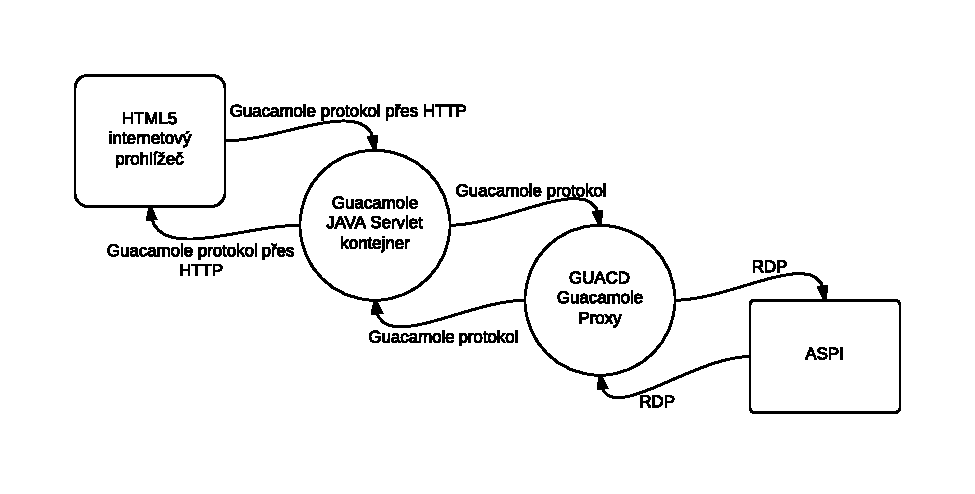
\includegraphics[scale=0.77]{img/architecture_overview.pdf}}
\caption{Pohled na architekturu řešení}
\end{figure}  

\section{Aplikace požadavků na prostředí Drupalu}

V Drupalu je využíváno několika základních ,,stavebních kamenů'', každý z nich může dle svého typu hluboce modifikován a přizpůsoben každému řešení. Základem jsou entity, uložené v databázi poskytují možnosti přidávání polí, podobně jako sloupců v databázi. Entity jsou několika moduly jádra Drupalu rozšířeny a poskytují funkcionalitu potřebnou k vytvoření webových stránek. Jmenovitě se jedná o uzly (node), které nám poskytují jednotlivé stránky a mají svou unikátní url adresu, a slovníky (taxonomy), které slouží ke kategorizaci obsahu a vytváření polí založených na výběru z dostupných prvků. Uzly i slovníky mohou být konfigurovány ve formě druhů obsahu, každý z nich s vlastními polemi nezávislými na ostatních entitách. Pole se stejným obsahem však mohou být sdílena pro ulehčení databázové struktury, do ktére se data reálně ukládají. Instance dostupných typů obsahu pak dostanou přidělené unikátní číslo v rámci všech entit, které určuje její data v databázi. Ne všechna pole musejí být zobrazena na stránce entity, nebo může pro jejich zobrazení být využito speciálních formátovacích technik, jako tabulek, či jiných výpisů.

Pro umístění obsahu na stránkách se využívají bloky (block), které lze přímo v UI umístit do předdefinovaných segmentů stránek (ty jsou definované v konfiguračních souborech tématu vzhledu viz. kapitola \ref{chap:implementace}).

Požadavky \cite{omaterna2013} poskytnuté Mgr. Maternou poskytují analýzu řešení, kterou však bylo potřeba aplikovat přímo na možnosti Drupalu a co nejvíce využít jeho možností - jednak pro samotnou implementaci řešení, ale také pro maximální ulehčení administrace a poskytnutí co nejvyšší míry soudržnosti skrze finální řešení projektu. Toho je dosáhnuto omezením vstupu a poskytnutím výběru z předdefinovaných možností (pokud je tento způsob řešení možný).

\subsection{Typy polí použitelné pro vlastnosti typů obsahu}
V drupalu existuje několik základních typů polí, které převážně fungují podobně jako datové typy v typických programovacích jazycích. Narozdíl od jednoduchých datových typů však poskytují navíc html formátování a mohou poskytovat i další nastavení. Formátování jde dále změnit pomocí přepsání základních formátovácích funkcí.

\subsubsection*{Text}
Poskytuje pole pro text s omezenou délkou bez možnosti vkládání html značek. Jeho obsah je zadáván pouze v jediném řádku a poskytuje pouze limitované možnosti nastavení, kterými je délka vstupního pole, či defaultní hodnota. 

\subsubsection*{Dlouhý text se souhrnem}
Narozdíl od typu pole Text může v tomto případě být text neomezeně dlouhý a obsahovat značky html kódu. Ty mohou být vkládány buď ručně a nebo automaticky formátovány pomocí \gls{wysiwyg} editoru. Zároveň je pro text možné vyplnit souhrn, který je ve specifických případech zobrazit, nebo se automaticky zobrazí zkrácená verze textu. Počet znaků je možné určit pro každou instanci pole zvlášť.

\subsubsection*{Hodnota slovníku}
V nastavení pole lze vybrat jeden z existujících slovníků. Jeho hodnoty pak jsou vypsány v jednom z dostupných formátů (radio/zaškrtávací tlačítka) a dle nastavení pak lze vybrat jen jedna, nebo více možností.

\subsubsection*{Logická hodnota}
Poskytuje pole pro logickou hodnotu - ano nebo ne. Pro hodnoty lze vybrat jednu z typicky použítelných nápisů (ano/ne, pravda/nepravda, checkmark/x), nebo definovat nápisy vlastní. 

\subsubsection*{URL adresa}
Kromě samotné adresy poskytuje možnost uložení dalších parametrů, podobně jako element <a> jazyka html. Mezi tyto parametry patří např. titulek, cíl a podobně.

\subsubsection*{Média}
Pro vkládání médií do systému je využit modul Media, který přidává komplexní řešení pro vkládání jakéhokoliv obsahu. Je možné vkládat dokumenty, soubory pdf, zvuk, obraz, či video a všechny tyto typy obsahu jsou uživately poskytovány v jednotném formátu.

\subsubsection*{Váha}
I když by se pro určení váhy produktu dalo využít jednoduchého číselného pole, jeden z rozšiřujících modulů poskytuje jednak speciálně využitelné pole pro výběr hodnoty a také pohledy na obsah a řadící funkce, které celou implementaci značně ulehčují.

\subsubsection*{Odkaz na entitu}
Důležitou vlastností většiny systémů je možnost propojení entit. Pro modelování těchto vztahů zde existuje typ pole odkaz na entitu, u kterého je možné vybrat typy entity, na které je daný typ obsahu navázán a způsob propojení. Za pomocí extra modulů lze také možné modelovat místo jednoduché asociace kompozici. V tom případě při smazání nadentity jsou smazány i všechny podentity. Lze také definovat, zda je možné pouze vytvářet nové podentity, či přidávat ty již existující.

\subsection{Typy obsahu}
Kdybychom si představili typy obsahu ve světě objektově orientovaného programování, všechny by dědily vlastnosti ze základní třídy \emph{Entita}. Těmito vlastnostmi jsou typ, ID a několik dalších důležitých pouze pro interní fungování redakčního systému. Z \emph{Entity} dědí třída \emph{Uzel}, která ji rozšiřuje o nadpis, URL a stav. Pro lepší představu jsou vztahy popsány na diagramu \ref{img:blabla}. Přímý předek typu obsahu je vždy zapsán v závorce za jeho názvem.

\begin{figure}[htp] \centering{
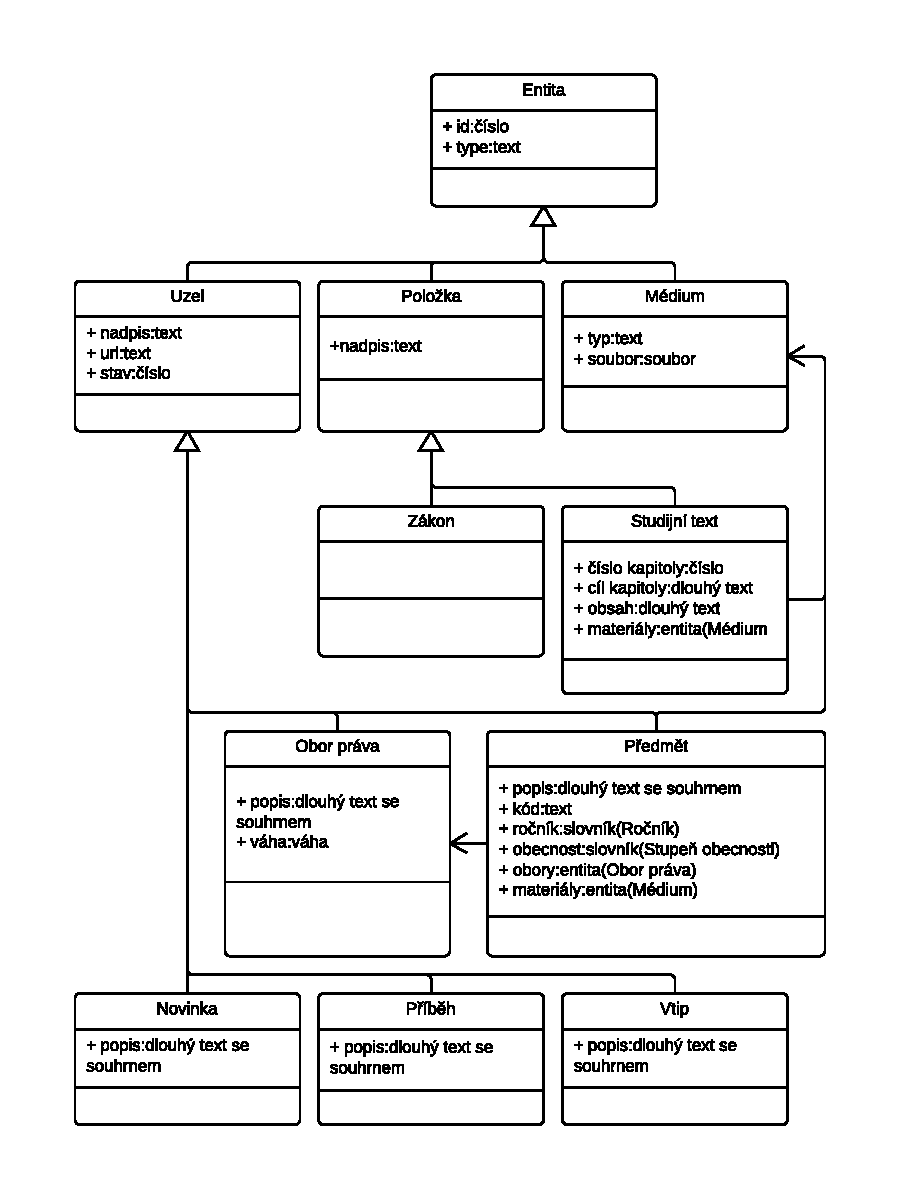
\includegraphics[scale=0.83]{img/class_diagram.pdf}}
\caption{Diagram tříd CMS systému}
\end{figure}  


\subsubsection*{Předmět \emph{(uzel)}}
Popisuje předmět vyučovaný v rámci fakulty ESF a tím vyjadřuje základní rozdělení celého portálu a slučuje hlavní část informací, o které se návštěvníci zajímají. Na stránce detailu předmětu je zobrazen ktátký popis, za kterým následuje tabulka se seznamem studijních textů a k nim vztahujících se materiálů. Materiály, které se vztahují přímo k předmětu jsou zobrazeny samostatně a celá stránka je uzavřana seznamem oborů, které se k danému předmětu vztahují.

\subsubsection*{Obor práva \emph{(uzel)}}
Předměty se mohou vztahovat k určitým oborům práva. Zatímco některé z nich se mohou dotýkat pouze jednoho z nich, jiné se mohou dotýkat všech. Proto je důležité tento vztah být vymodelovat a uživatelům poskytnout možnost se v tomto jednoduše orientovat a přecházet mezi obsahem, který jej právě zajímá. Na stránce oboru práva je zobrazen popis oboru a tabulka se seznamem předmětů, které se k němu vztahují.

\subsubsection*{Studijní text \emph{položka}}
Studijní text obsahuje informace vztahující se k jednomu celku výuky, typicky k jedné přednášce. Lze definovat zkrácený cíl přednášky, přidat k ní materiály a určit její pořadové číslo. U všech materiálů je vhodné zadat název pro správné zobrazení v tabulce detailu předmětu, na kterém se zobrazuje seznam těchto entit.

\subsubsection*{Zákon \emph{položka}}


\subsubsection*{Příběh \emph{(uzel)}}
Pro odreagování studentů je v jednom ze segmentů stránek zobrazován příběh z právního prostředí. 

\subsubsection*{Vtip \emph{(uzel)}}
V postranním panelu lze zobrazit vždy aktuální vtip z právního prostředí, který také slouží k odreagování studentů. \\

\subsubsection*{Novinka \emph{(uzel)}}
Na stránkách jsou publikovány novinky (aktuality) týkající se buď portálu samotného, fakulty ESF, či jakýchkoliv dalších relevantních událostí. Novinky jsou zobrazovány na úvodní stránce. \\

\subsection{Slovníky}

Pro kategorizaci a pro výběr možností bylo v požadavcích identifikováno několik slovníků. Díky vztahu k entitě (slovník také dědí vlastnosti entity) může také pro své hodnoty definovat pole a tím rozšířit jejich funkcionalitu a množství informací.

\subsubsection*{Stupeň obecnosti}
Pro řazení oborů je potřeba uložit jejich obecnost, která je vyjádřena v několika stupních, které mohou být v případě potřeby rozšířeny. Každé entitě může být přiřazen jeden stupeň obecnosti.\\

\begin{list}{-}{Pole}
  \item Váha (váha) \\
    číselná hodnota použitelná k řazení
\end{list}

\begin{list}{-}{Hodnoty}
  \item Velmi obecný \emph{(váha = 0)} 
  \item Středně obecný \emph{(váha = 1)}
  \item Málo obecný \emph{(váha = 2)}
\end{list}

\subsubsection*{Ročník}
Pro případné budoucí úpravy systému, či filtrování, je vhodné u předmětu vyplnit i ročník, ve kterém je vyučován. S ohledem na opakování předmětů může každé entitě přiřazeno neomezené množství ročníků (i žádný). \\

\begin{list}{-}{Hodnoty}
  \item 2012/13
  \item 2013/14
  \item 2014/15
\end{list}
